\begin{center}

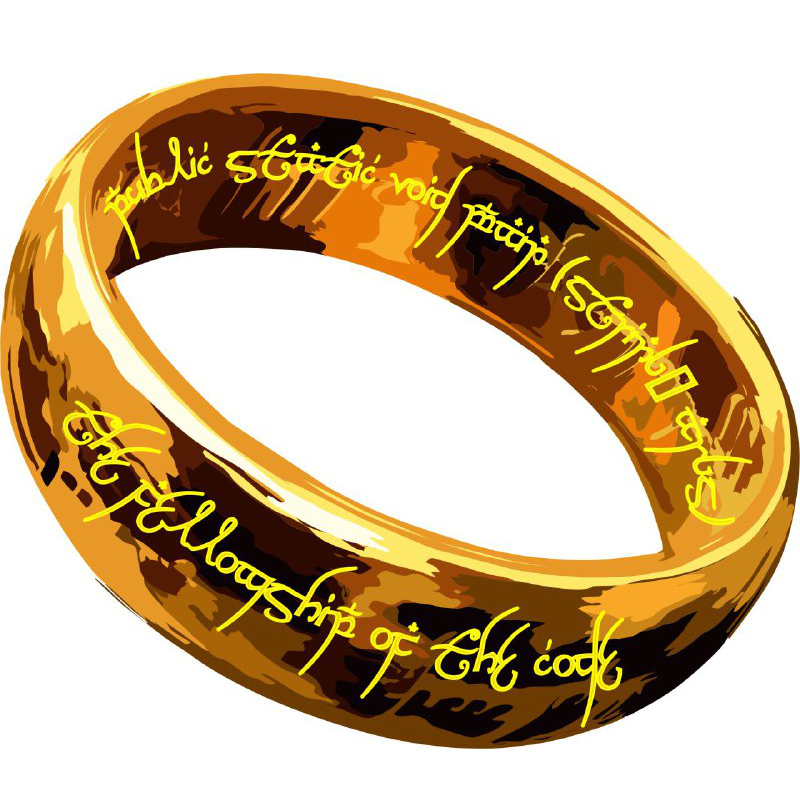
\includegraphics[width=1em]{../../Template/icone/logo_fotc.jpg}
\begin{large} \textbf{\gruppoLink} \end{large}
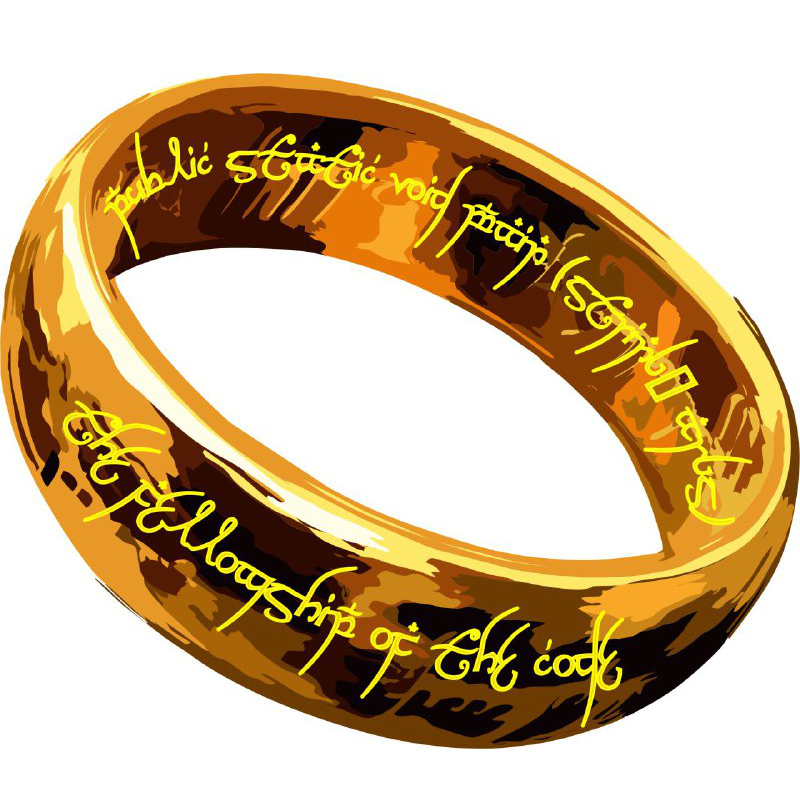
\includegraphics[width=1em]{../../Template/icone/logo_fotc.jpg}
\vspace{0.2em}

\hrule
\vspace{3em}


\includegraphics[keepaspectratio = true]{../../Template/icone/logo.jpg}

%Prima pagina senza intestazione né piè di pagina	
\thispagestyle{empty}

%Le informazioni del documento sono ancorate a fine pagina
\vfill

%Copertina
\begin{center} 
  \begin{Huge}
  {\fontsize{15mm}{20mm}\selectfont \progetto} 
  \end{Huge}
\end{center}

\begin{Huge} \documento \end{Huge}

\begin{center}
\textbf{Informazioni sul documento} \\ \vspace{2em}
\small
\begin{tabular}{r|l}
	\textbf{Nome Documento} & \nomedocumentofisico \\
	\textbf{Versione}	& 1\\
	\textbf{Data di Creazione} & \datacreazione\\
	\textbf{Data ultima modifica} & \datamodifica\\
	\textbf{Stato} & \stato \\
	\textbf{Redazione}	& \redazione\\
	\textbf{Verifica}	& \verifica\\
	\textbf{Approvazione}	& \approvazione\\
	\textbf{Uso}  & \uso\\
	\textbf{Distribuzione} & \gruppo \\
	\textbf{Destinato a}  &  \destinateTo \\
	\textbf{Email di riferimento} & \email
\end{tabular}
\end{center}

\normalsize
%Sommario
\textbf{Sommario\\} 
Documento contenente le norme di progetto che il gruppo \textit{\gruppo} seguirà durante tutte le fasi di realizzazione del prodotto \textit{\progetto}.

%\vfill %cosa fa?
\end{center}
\clearpage
